\fancychapter{State of the art}
\label{ch:state_of_the_art}
This section provides insight of work done in several research areas that are related to the project. In section ~\ref{sec:self_organizing_maps}, work done using \ac{SOM} maps will be described. Section ~\ref{sec:topic_detection_on_twitter} and~\ref{sec:data_mining_in_twitter_} are dedicated to data clustering and to data mining specifically on Twitter~\footnote{http://www.twitter.com}.

\section{Self-Organizing Maps} 
\label{sec:self_organizing_maps}
\ac{SOM} are used in a wide area of applications, from authentication systems~\cite{Dozono2012} through network intrusion detection~\cite{intrusion_som} and speech recognition and analysis~\cite{phonetic_typewiter}. In this section we highlight some of their applications.

\subsection{The Geo-SOM} 
\label{sub:types_of_soms}
The Geo-SOM, by~\citet{Bacao2005}, applies the first law of geography “Everything is related to everything else, but near things are more related than distant things."~\cite{citeulike:612692} to the \ac{SOM} algorithm. In this case, the winning neuron is chosen in a radius defined by the geographic-coordinates of the data, forcing units that are close geographically to be close in the output space.

The algorithm works by defining a variable $k$ which is used as a "geographical tolerance" that forces the winning neuron to be geographically near the input pattern. When $k=0$, the winning neuron is forced to be the unit geographically closest to the input data, whilst $k$ increases, the tolerance for data with further geographic coordinates, increases as well. $k$ is a geographic radius applied in the output space. When the radius exceeds the size of the output space, every unit is eligible to be the winning neuron, and therefor, we have a regular \ac{SOM}.

The selection of the winning neuron is done in two steps. First, geographic neurons inside the tolerance $k$ with the input data as a center are selected. Only after that, comparisons are made with the rest of data present in the input data. The representation of the Geo-SOM can be seen in Figure~\ref{fig:geo_som}, where the units considered for the best match are defined by a sort of geographic radius defined by $k$, whilst in the original \ac{SOM}, the winning neuron could have been any of the units presented on the figure.

The Geo-SOM approach to the alteration of the default \ac{SOM} algorithm is specially interesting due to the fact that this thesis objective is also to give relevance to data patterns that are not located in the same space as the trained data. In a way, what we are trying to achieve is similar to the work by~\citet{Bacao2005} but changing the geographic relevance in data by a social relevance.
\begin{figure}[tb]
  \begin{center}
    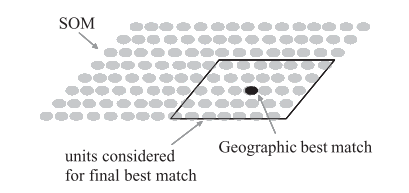
\includegraphics[]{images/6_geo-som.png}
  \end{center}
  \caption{Geo-SOM structure, where the units considered to be the winning neuron are constrained by the geographic coordinates of the data, from~\citet{Bacao2005}}
  \label{fig:geo_som}
\end{figure}

\subsection{Detecting Hidden Patterns on Twitter Usage} 
\label{sub:detecting_hidden_patterns_on_twitter_usage}
Cheon and Lee~\citep{Cheong2010} analyzed hidden patterns in the usage of twitter. In their study, they started by collecting data from the twitter API of different kinds of topics like "2009 Iran Election" and "iPhone 3.0 OS launch". They made multi level signal extraction, not only from information directly present on the tweet, but also by cross referencing with other social websites and with the twitter user profile information. The signals retrieved from the social network can be seen in Table ~\ref{tab:twitter_signals}.

\begin{table}[H]
  \caption{Twitter Signals}
  \label{tab:twitter_signals}
  \begin{center}
    \begin{tabular}{|l|}
      \hline
      \textbf{Twitt Corpus}  \\
      \hline
      Tweet Size \\
      \hline
      Replies \\
      \hline
      Re-tweets \\
      \hline
      Hashtags  \\
      \hline
      \specialcell{Presence of URIs and \\ Type of linked content} \\
      \hline
      Type of Device   \\
      \hline
      Tweet Location  \\
      \hline                 
      \hline                 
      \textbf{Twitter Profile} \\ 
      \hline
      Account Age   \\
      \hline
      Gender     \\
      \hline
      Country \\    
      \hline
      frequency of posts \\
      \hline
      Friends to followers ratio \\ 
      \hline
      Number of  customizations \\   
      \hline
      \hline
      \textbf{External Sources} \\
      \hline
      Other Social Network Accounts   \\
      \hline
      Type of website\\ 
      \hline
    \end{tabular}
  \end{center}
\end{table}

By applying a \ac{SOM}, they could find four demographical clusters during the Iran 2009 Election. The first cluster was characterized by young web-based Iranians, with twitter accounts not older than three months with a high frequency of replies. The second cluster was mainly compound of web users from Iran accounts older that three months. The third cluster had Iranian users with mobile clients with large texts clearly trying to raise awareness. The fourth and final cluster represented the users around the world trying to raise awareness about the issue by sharing tweets with URIs.
Looking at their analysis about the topic "2009 Iranian Election", it is clear to see that it was possible to describe the type of users represented in the social network and the way they interact with it.

On the iPhone 3.0 OS launch, it was possible to find three main clusters. The first cluster was characterized by male users, accounts older than 90 days, coming from countries where the iPhone is marketed, with high adoption of social media clearly representing the target market of the iPhone or its customers. The second cluster had new accounts with higher rate of followers to followees, high frequency of posts per day, presence of URI linking to technology blogs or websites, no country or gender specified meaning that this cluster was clearly composed by news aggregators and technological news websites. Inside the second cluster, there was a sub-cluster of Japanese users which represents the high rate of iPhone adoption in Japan. Finally, the third cluster was clearly spammer accounts that where eventually deleted after a couple of months, characterized by popular social connections, posting more than fifty tweets a day with external URIs and the accounts were not older than a day or so.

In conclusion, it was possible to detect Twitter usage patterns, and specifically, detect spammers before they were banned from the social network. 

\subsection{WEBSOM}
\label{sub:websom}
\citet{honkelawebsom} developed a new approach to automatically order arbitrary, free from textual, document collections, using two different SOMs. The first \ac{SOM} is called word category map and it's used to find words that have similar meaning, while the second \ac{SOM}, called document map, is the one actually used to cluster the documents. 

The WEBSOM was not based on keywords and boolean expressions, instead, words with the same meaning are encoded in a word category map (Fig~\ref{chp3:img3}), where placement and frequency in documents is taken into account. This way it is possible to remove words with similar meaning --- greatly reducing the \ac{VSM} size  making it possible to train the document map in a scalable way.
                                                                                                          
\begin{figure}[htpb]
  \centering
  \subfigure[The word cathegory map, a SOM where word frequency and placement is used for encoding text]{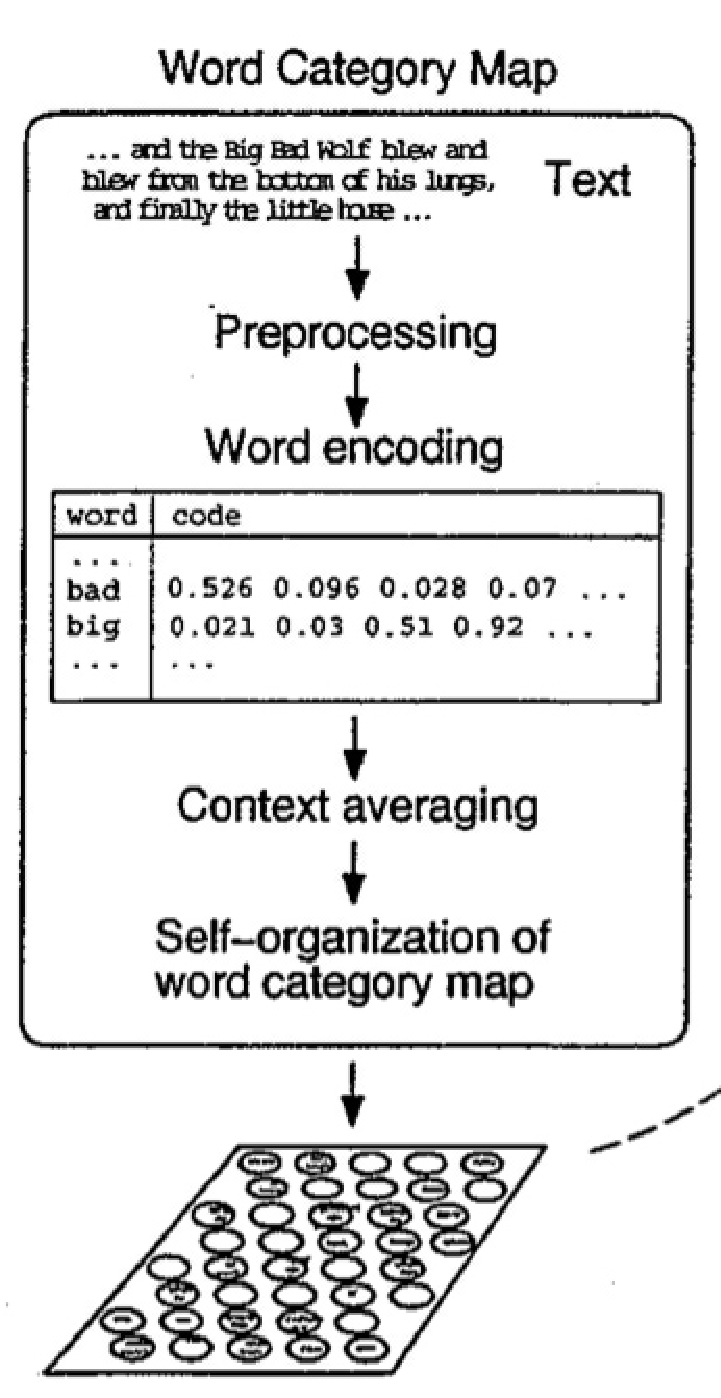
\includegraphics[scale=0.5]{./images/wordclusteringmap.pdf}\label{chp3:img3}}
  \hspace*{0.3cm}
  \subfigure[The document map, organized based on documents enconded with the word cathegory map.]{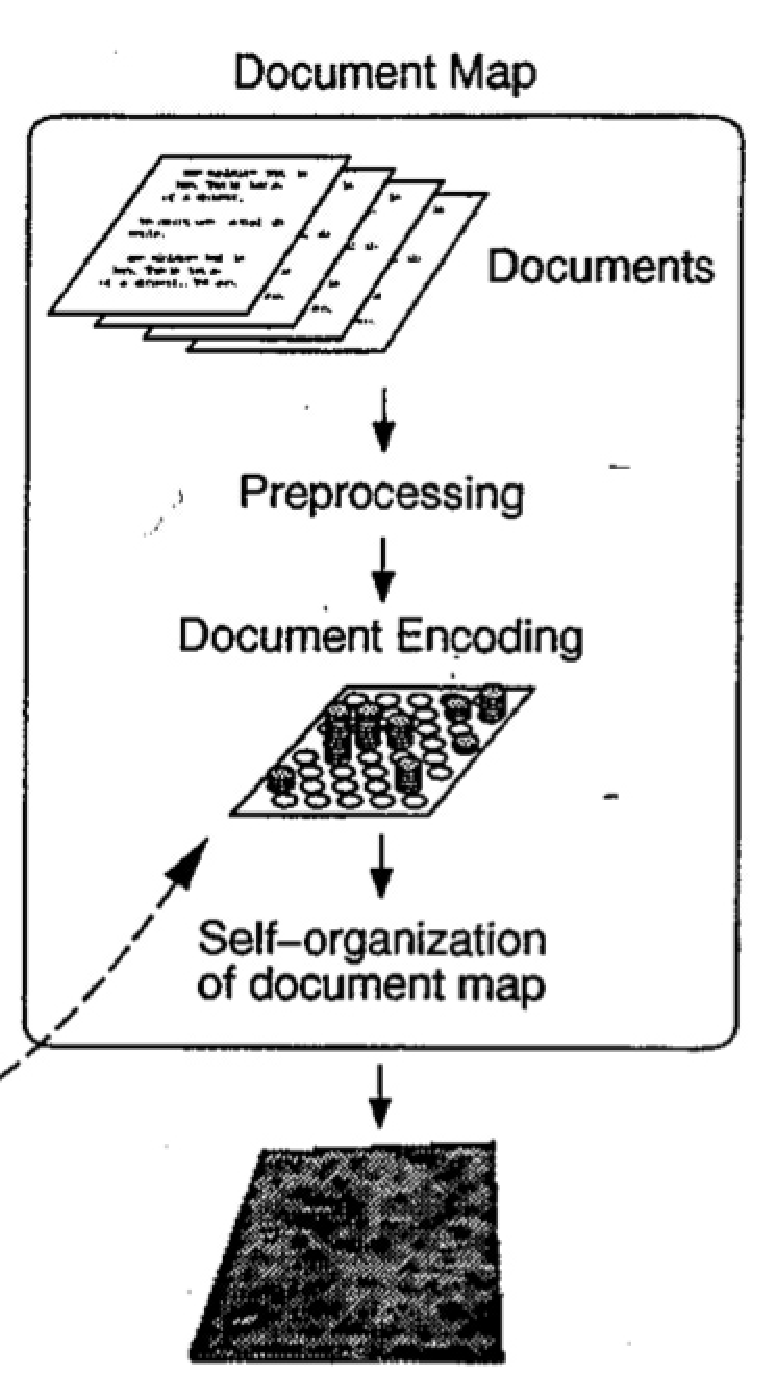
\includegraphics[scale=0.5]{./images/wordclusteringmapmap.pdf}\label{chp3:img4}}\\
  \caption{Basic architecture of the WEBSOM method, from~\cite{honkelawebsom}}
  \label{fig:websom}
\end{figure}

\section{Twitter Data Mining and TTD} 
\label{sec:data_mining_in_twitter_}

In this subsection, we will focus on work done on the Twitter social network in order to leverage insights on how the public data available from the website can be explored. 

\subsection{Topic and Trending Detection} 
\label{sub:real_time_topic_and_trending_detection}
%\section{Topic Detection and Tracking with Clustering} 
%\label{sec:topic_detection_on_twitter}

~\citet{allan2002topic} defined \ac{TDT} as “a constantly arriving stream of text from newswire and from automatic speech-to-text systems that are monitoring selected television, radio, Web broadcast news shows. Roughly speaking, the goal of \ac{TDT} is to break the text down into individual news stories, to monitor the stories for the events that have not been seen before, and to gather stories into groups that each discuss a single news topic".

Nowadays, due to the rapid adaptation of people to always be on-line, through the usage of cellphones on the move, desktops at work and even TV at home, the increase of user generated content has increased tremendously in latest years. In 2006, 35\% of on-line adults and 57\% of teenagers created content on the Internet \footnote{ Data source: http://www.pewinternet.org/Presentations/2006/UserGenerated-Content.aspx}, which in "Internet Years" was ages ago. 

The challenge of \ac{TDT} is evermore focused on online generated documents, and in new forms to be able to track and categorize all the information that is continuously being generated.
Many \ac{TDT} techniques have been proposed,  a significant amount of them rely on the \ac{TF-IDF}~\cite{Baeza-Yates:1999:MIR:553876}. Because tweets are very small, often with typos or slang words, and because the same tweet might be written in multiple languages, \ac{TF-IDF} is not particularly adequate for topic detection on twitter. In this subsection, we will take a look at multiple methods of topic detection in general, and also specifically on the Twitter social network.

%With amount of content increasing, new real-time and scalable algorithms are needed in order to make sense of all this data.
~\citet{Cataldi2010} proposed a new technique for emerging topic detection that permits real-time retrieval of the most emergent topics expressed by a community on Twitter. Their work applies the PageRank algorithm~\cite{Pagerank1998} to the users follower/followee relationship, in order to find the most influential users on the network. Then, the most trending topics are calculated, by relating social influence, word co-occurrence and time frame. In the end, an interface was created where it would be possible to navigate, through hot topics in a given time frame. Topic labeling was not automatic and was implicit by the time frame of an event.
%REMOVEDBYPAVEL
%, if two highly social events would occur in the same time frame with word relations the results could be interpreted as the same, for example if a political candidate would win the elections at the same of an important sports club would win a specific cup, the word \emph{win} could be trending at the same time for two different topics and due to high temporal dependency they could be interpreted as the same topic.

~\citet{Weng2010} also used the PageRank algorithm to find the most influential twitter users on a certain topic. However, using a different approach, they represent each twitter user as a bag of words comprising of all the tweets that they have posted, and applied \ac{LDA}~\cite{Blei2003} in order to find topics in which users are interested in. Finally, it was possible to prove that follower/followee relations on twitter are not just casual, but that people actually follow other people to whom they have some resemblance or common interest. This concept is called homophily and will be further explored on this thesis.
 
\subsection{Tweets Implicit Data} 
\label{sub:the_tweet}
Tweet retrieval and analysis is a double edged problem. On one side, the tweet is really small, which makes it almost impossible to retrieve any actual sense from it. On the other hand, the amount of tweets generated per day is around 140 million\footnote{https://blog.twitter.com/2011/numbers}, which means that it is very hard to do a deep analysis of the semantics and content of individual tweet, and that only the more appropriate signals should be evaluated.
For this reason, \citet{Tao2012} evaluated how the multiple signals that could be retrieved, directly or indirectly, from the tweet corpus could mean that a tweet is relevant for a determined topic. In their work, they present premises that seem intuitively true and proves they actually are relevant through a comparison of multiple precision and recall values. Their results on feature comparison are summarized in Table~\ref{tab:tao_table}. The first column consists of all the made hypothesis categorized by type, and the second column tells if the data used actually influenced in precision and recall results. \citet{Tao2012} also compared results, of topic characteristics, concluding that distinction between local and global events as well as temporal persistence proved to not be relevant on relevance prediction.

\begin{table}[tb]
  \caption{~\citet{Tao2012} tweet characteristics hypothesis versus influence}
  \label{tab:tao_table}
  \begin{tabularx}{\textwidth}{|X|l|}
  \hline
  \textbf{Hypotheses} & \textbf{Influence of Features} \\
  \hline
  \hline

  {\bf Syntatical} &  \\
  \hline
  Tweets that contain hashtags are more likely to be relevant than tweets that don't & Not Important \\
  \hline
  Tweets that contain an URI are more relevant that tweets that don't  &Important \\
  \hline
  Tweets that are replies to other tweets are less relevant & Important \\
  \hline
  The longer the tweet is the more relevant it is & Not Important\\
  \hline
  \hline

  {\bf Semantic}  &  \\
  \hline
  
  The more the number of entities the more relevant a tweet is  & Important \\
  \hline
  Different types of entities are of can have different amount of interest to a give topic  & Important \\
  \hline
  The greater the diversity of concepts mentions in a tweet the more likely for it to be relevant & Important \\
  \hline
  The relevance of a tweet is determined by its polarity & Important \\
  \hline
  \hline

  {\bf Contextual} &  \\
  \hline
  The lower the temporal distance between a query and the creation of a tweet the more relevant the tweet is  & Not Important \\
  \hline
  The more the number of tweets created by a user the more relevant one of his tweets will be & Not Important \\
  \hline
  \end{tabularx}
\end{table}

~\citet{McCreadie2013} also approached the issue of having very little content on tweets in order to categorize them, and tried to solve the problem by applying the content of linked URIs into the tweet body in order to improve precision and recall. The best fitting approach was using Field-Based weighting, where for each tweet a new document is created, which contains two fields: the terms in the tweet and the terms in the linked document. 
Afterwards a learning to rank algorithm called PL2F~\cite{macdonald2008} is used against the dataset from "Trec Microblog2011" in order to find the best weighting. 
With this model they were able to improve precision in an order of 0.9, over only analyzing the text contained in the tweets. 

\subsection{Tweeter Natural Language Processing}
\label{sub:tweeter_natural_language_processing}
Using standart \ac{NLP} tools on tweets has been extremely unreliable, due to the fact that microbloging text tends to be full of abbreviations, emojis and smiles . Recently, ~\citet{owoputi13improvedparth} published a \ac{NLP} library, specific for twitter. As shown in Figure~\ref{fig:nlp}, ARK Tweet \ac{NLP} can tag words that are only used in social networks. The tagger was built using maximum entropy Markov model, where a tag is assigned to a word based on the entire tweet text, and the tag assigned to the word to its left. ~\citet{owoputi13improvedparth} state that the tagger has a 93.2\% accuracy. 
By using \ac{NLP} tools, it is possible to reduce the dimension of \ac{VSM} space by only choosing words that are relevant, like common nouns, hashtags and proper nouns. This will not only yield better results by removing tweets that have no content, and therefor, cannot be categorized, but will also increase performance during training due to the reduced dimensions caused by less use of words.
\begin{figure}[htpb]
  \centering
  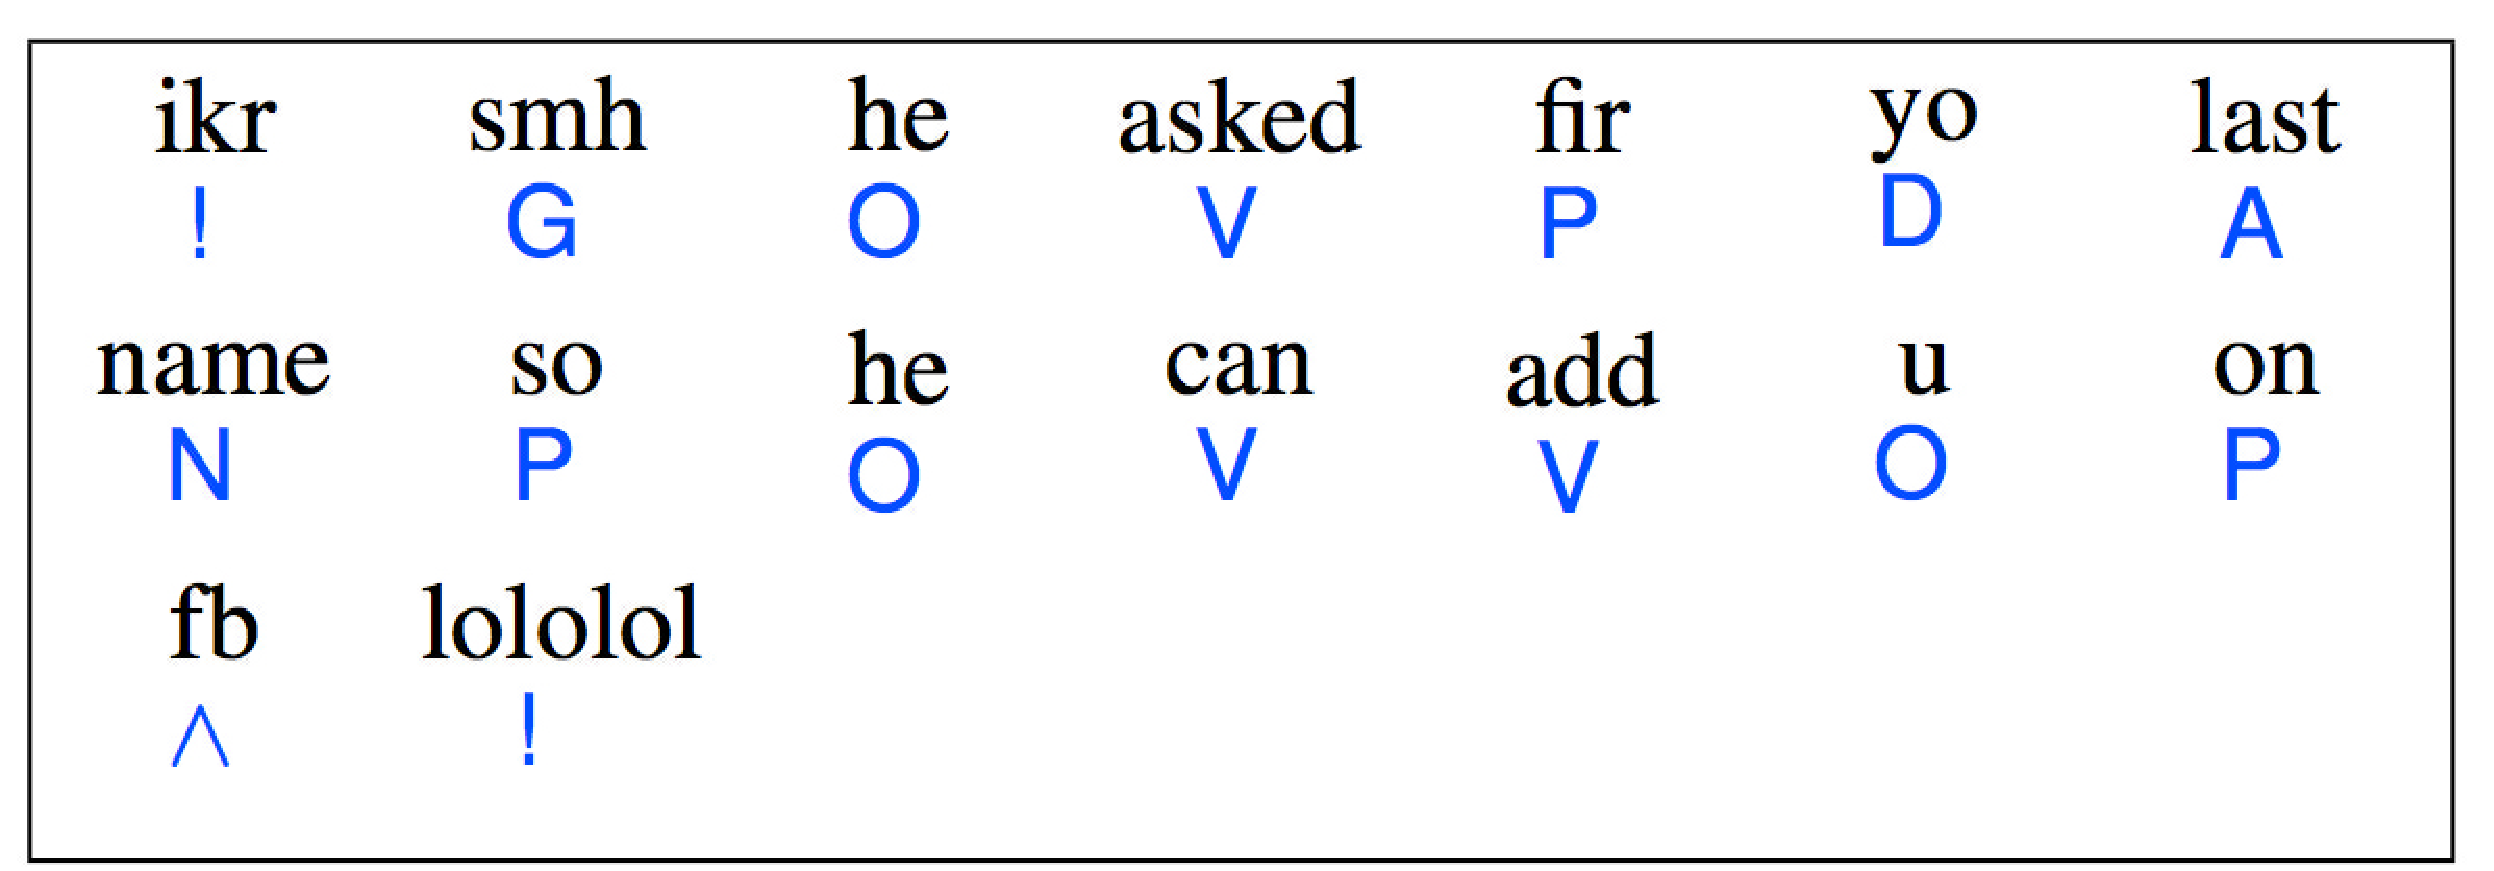
\includegraphics[width=0.6\linewidth]{./images/nlp.pdf}
  \caption{Tweet automatically tagged with ARK Tweet NLP. ! stands for interjection, while V stands for verbs and D for determiner. The full table of tags can be found in~\cite{owoputi13improvedparth}.}
  \label{fig:nlp}
\end{figure}

\subsection{Rapidly Changing Trends} 
\label{sub:real_time_}
Due to the real time nature of Twitter, using typical retrieval model, that relies on term frequency models like Okapi BM25 or language modeling cannot be applied, as stated by~\citet{Lin2012}. The study of topic endurance on the social network proved that topics are presented in bursts of queries and mentions. In addition the typical usage of twitter for search is not the same of Google. When users are searching on twitter, they want to find out what is happening in that moment, meaning that classification techniques based on past events cannot respond this kind of problem. As stated by~\citet{Lin2012}, this problem has not yet been solved at Twitter (or anywhere else at the time of writing this report), and issues a new kind of data analysis approach that was not taken into consideration in the past. 

This effect of rapidly changing topics and queries based on real time events was named "Churn", and can be clearly seen in Figure ~\ref{fig:churn}.

By including social features into clustering algorithms, it might be possible to discover interesting rising topics to a specific specific user, by categorizing them through a trained \ac{SOM}.

\begin{figure}[tb]
  \begin{center}
    \noindent\makebox[\textwidth]{
      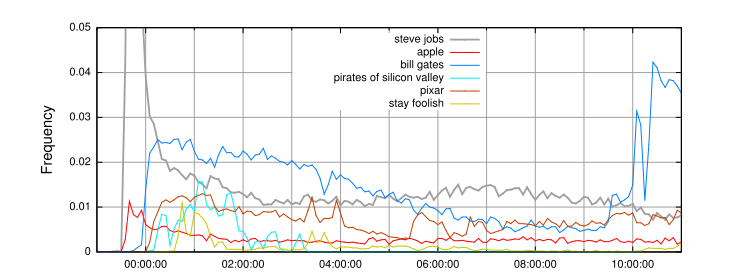
\includegraphics[width=13cm]{images/7_churn.png}
    }
  \end{center}
  \caption{The Churn effect: Frequencies of queries related to Steve Jobs death over a 12 hour period in 5-minute intervals, normalized to the total number of queries in the interval. At its peak, the query “steve jobs” reaches 0.15 (15\% of the query stream); Graph taken from~\cite{Lin2012}}
  \label{fig:churn}
\end{figure}


\section{Summary}
%TODO Sumarize the state of the art
Ending section summarizing the chapter is typically a good idea.

Ensure that the next chapter starts in a odd page
\cleardoublepage 
